% !TEX encoding = UTF-8 Unicode
\documentclass{article}

\usepackage{polski}
\usepackage[utf8]{inputenc}
\usepackage{subfig}
\usepackage{graphicx}

\usepackage[a4paper, left=2.5cm, right=2.5cm, top=3.5cm, bottom=3.5cm, headsep=1.2cm]{geometry}

\linespread{1.3}
\begin{document}
	
	\begin{titlepage}
		\centering
		{\scshape\LARGE Politechnika Wrocławska \par}
		{\scshape\Large Katedra Informatyki Technicznej\par}
		
		\vspace{1cm}
		{\scshape\Large Inżynieria Oprogramowania\par}
		\vspace{1.5cm}
		{\huge\bfseries Zapoznanie się z wybranym narzędziem UML - wprowadzenie do UML\par}
		\vspace{2cm}
		{\Large\itshape Magdalena Biernat\par}
		{\Large\itshape Mateusz Bortkiewicz\par}
		\vfill
		Opiekun\par
		prof. dr hab. inż. Jan Magott 
		
		\vfill
		{\large \today\par}
	\end{titlepage}
	\newpage
	
	\section{Wprowadzenie}
	Sprawozdanie dotyczy drugich zajęć. Na tych laboratoriach zaczęliśmy swój projekt. 
	
	\subsection{Cel laboratorium}
Specyfikacja wymagań, zdefiniowanych w ramach laboratorium 2, za pomocą diagramów przypadków użycia – tworzenie modelu
przypadków użycia 
	
	\subsection{Plan pracy}
	Zadania wykonaliśmy wg instrukcji 3:

	\begin{itemize}
		\item Wykonanie diagramu przypadków użycia.
		\item Zdefiniowanie aktorów.
		\item Wykonanie scenariuszy przypadków użycia.
	\end{itemize}
\newpage
	\section{Laboratorium}
	\subsection{Wykonanie diagramu przypadków użycia}
	\newpage
	\subsection{Zdefiniowanie aktorów}
\begin{figure}
	\centering
	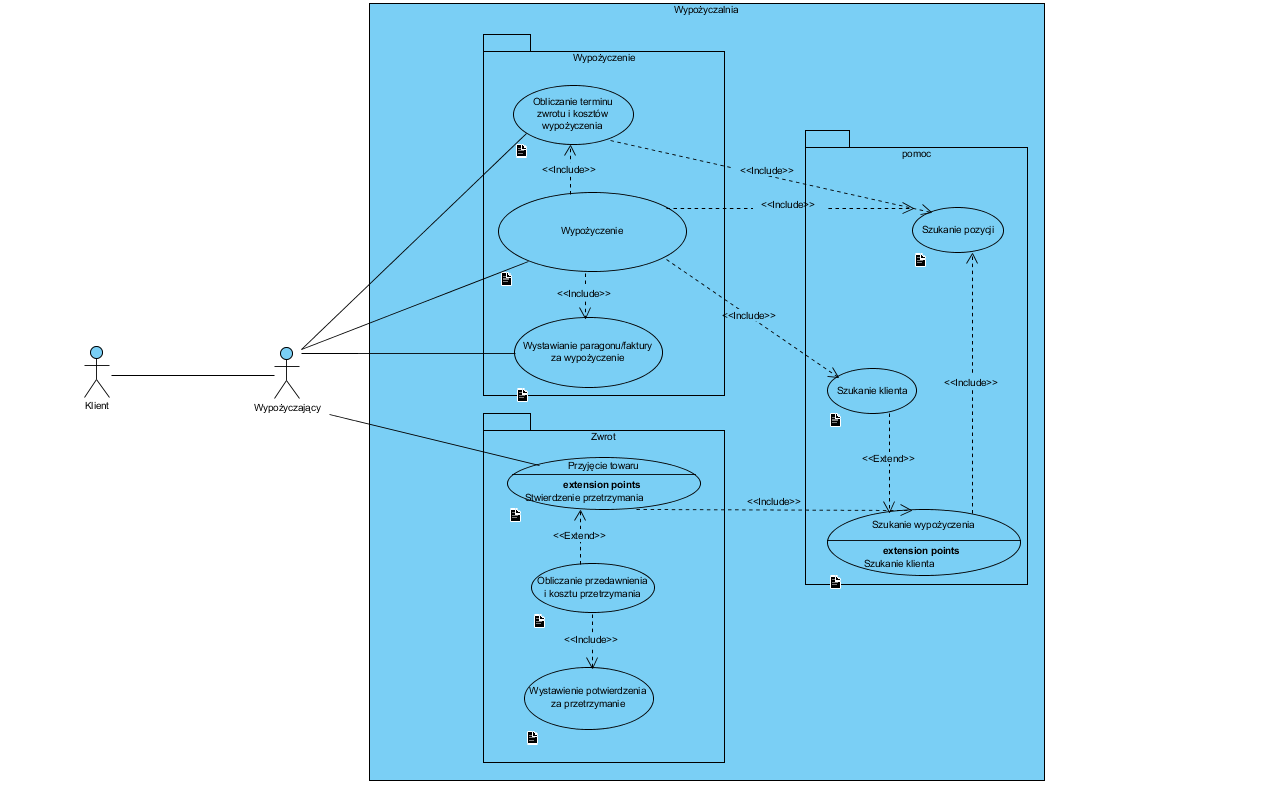
\includegraphics[height=10cm]{diagram.png}
	\caption{Diagram przypadków użycia}
	\label{fig:obrazek 1}
\end{figure}
\begin{tabular}{|rp{0,25\linewidth}|lp{0,25\linewidth|} \hline 
	AKTOR & OPIS & PRZYPADKI UŻYCIA   \\
	\hline
	Klient & Klient wypożycza za pośrednictwem wypożyczającego &    \\
	\hline
	Wypożyczający & Wypożyczający wypożycza klientowi towar korzystając z aplikacji.  Aplikacja wylicza termin i koszt wypożyczenia Może też wyszukiwać klienta i artykuły. Może też wystawić rachunek lub fakturę. Wypożyczający przyjmuje również zwroty i alikacja wylicza wtedy przedawnienie i koszt przetrzymania. 
	PU Obliczanie terminu zwrotu i kosztów wypożyczenia 
	PU Wypożyczenie 
	PU Wystawienie paragonu/faktury za wypożyczenie 
	PU PUPrzyjęcie towaru
	PU Obliczenie przedawnienia i kosztu przetrzymania
	PU Sukanie pozycji
	PU Szukanie klienta
	PU Szukanie wypożyczenia \\
	\hline 
\end{tabular}
	\newpage
	\subsection{Wykonanie scenariuszy użycia}	
\LARGE 	Wypożyczenie 
\Large	Obliczanie terminu zwrotu i kosztów wypożyczenia \newline
\normalsize	Cel: Obliczenie terminu zwrotu i kosztów wypożyczenia na podstawie informacji od klienta i wskazanych pozycji.\newline
	WS: Może być wywołany przez Wypożyczającego, musi być wywołany przy Wypożyczeniu \newline
	WK: Podanie terminu zwrotu i kosztów wypożyczenia\newline
	Przebieg:
\begin{enumerate}
	\item Odwołanie się do produktu w bazie danych
	\item Zwrot terminu i kosztów wypożyczenia na podstawie danych produktu
\end{enumerate}
\Large Wypożyczenie
\normalsize
\begin{enumerate}
	\item[Cel:] Wypożyczenie klientowi produktu/produktów. 
	\item[WS:] Produkt musi być niewypożyczony 
	\item[WK:] Wypożyczenie musi być zarejestrowane w systemie 
\end{enumerate}
Przebieg:
	\begin{enumerate}
		\item Szukamy klienta.
		\item Następuje obliczenie terminu zwrotu i kosztów wypożyczenia.
		\item Klientowi zostają przypisane pozycje – następuje wypożyczenie
		\item Następuje wystawienie paragonu/faktury za wypożyczenie.
	\end{enumerate}
\Large	Wystawienie paragonu/faktury za wypożyczenie 
\normalsize
\begin{enumerate}
	\item[Cel:] Wystawienie klientowi paragonu/faktury
	\item[WS:] Wypożyczenie musi być zarejestrowane w systemie
	\item[WK:]  Paragon/faktura musi być zarejestrowana w systemie.
\end{enumerate}
	Przebieg:
	\begin{enumerate}
		\item Na podstawie danych z wypożyczenia jest generowany dokument
		\item 	Dokument jest zapisany do systemu
	\end{enumerate}
\LARGE	Zwrot \newline
\Large	Przyjęcie towaru\newline
\normalsize
\begin{enumerate}
\item[Cel:] Zwrot wypożyczonego uprzednio towaru
	\item[WS:] Towar musi być wypożyczony
	\item[WK:]  Towar będzie dostępny do wypożyczenia, a klient rozliczony z wypożyczalnią.
\end{enumerate}
	Przebieg:
	\begin{enumerate}
		\item Znalezienie wypożyczenia na podstawie wypożyczonej pozycji.
		\begin{enumerate}
			\item [1.1] Opcjonalnie za pomocą danych klienta 
		\end{enumerate}
		\item Jest wystawione potwierdzenie zapłaty za przetrzymanie
			\begin{enumerate}
			\item [2.1] Opcjonalnie za pomocą danych klienta 
		\end{enumerate}
		\item Towar jest zwrócony do wypożyczalni.
	\end{enumerate}
\Large	Obliczanie przedawnienia i kosztu przetrzymanie\newline
\normalsize
\begin{enumerate}
	\item[Cel:] Obliczanie przedawnienia i kosztów przetrzymania
	\item[WS:] Termin wypożyczenia musi być przekroczony
	\item[WK:]  Wystawienie potwierdzenia zapłaty za przetrzymanie wypożyczalnią.
\end{enumerate}
	Przebieg:\newline
	\begin{enumerate}
		\item Pobierana jest przetrzymana pozycja i w zależności od niej – obliczana kwota przetrzymania
		\item Następuje generowanie dokumentu
		\item Dokument jest zapisany do systemu
	\end{enumerate}
	\Large	Wystawienie potwierdzenia za przetrzymanie \newline
	\normalsize
	\begin{enumerate}
		\item[Cel:] Wystawienie potwierdzenia za przetrzymanie
		\item[WS:] We wskazanym wypożyczeniu musi wystąpić przedawnienie
		\item[WK:] Wystawienie potwierdzenia zapłaty za przetrzymanie
	\end{enumerate}
	Przebieg:\newline
	\begin{enumerate}
	\item Zostaje pobrany termin i kwota przedawnienia 
		\item Następuje generowanie dokumentu
		\item Dokument jest zapisany do systemu
	\end{enumerate}
\LARGE	Pomoc\newline
\Large	Szukanie wypożyczenia\newline
\normalsize
\begin{enumerate}
	\item[Cel:] Wyszukanie interesującego nas wypożyczenia
	\item[WS:] Musi zostać wprowadzona dana do wyszukiwania: np. tytuł, kod kreskowy etc albo dana klienta
	\item[WK:] Zwrócona zostaje interesujące nas wypożyczenie
\end{enumerate}
Przebieg:
\begin{enumerate}
	\item Zostaje zeskanowany kod kreskowy 
	\begin{enumerate}
		\item [1.1] Jeśli jest nieczytelny to wyszukujemy dane klienta
	\end{enumerate}
	\item Jeśli pozycja jest niewypożyczona, zwracamy informację o braku wypożyczenia
	\item Jeśli jest wypożyczona, to zwracamy wypożyczenie.
\end{enumerate}
	\Large	Szukanie klienta\newline
	\normalsize
	\begin{enumerate}
		\item[Cel:] Wyszukanie klienta
		\item[WS:] Musi zostać wprowadzona dana klienta: Nazwisko, Pesel albo telefon
		\item[WK:] Zwrócenie konta klienta
	\end{enumerate}
	Przebieg:
	\begin{enumerate}
		\item Zostaje pobrana dana
		\item Jeśli brak takiego klienta, zwracamy informację o braku konta
		\item Jeśli występuje klient to zwracamy jego konto
	\end{enumerate}
		\Large	Szukanie pozycji\newline
		\normalsize
	\begin{enumerate}
		\item[Cel:] Wyszukanie pozycji, instancji tytułu artykułu
		\item[WS:]Musi zostać wprowadzona dana do wyszukiwania: Kod kreskowy, nazwa albo autor
		\item[WK:] Zwrócenie interesującej nas pozycji
	\end{enumerate}
	Przebieg:
	\begin{enumerate}
		\item Zostaje pobrana dana
		\item Na podstawie danej zwracamy pasującej do niej pozycje książek
		\begin{enumerate}
			\item [2.1] Jeśli brak pozycji to zwracamy informację o braku pozycji
		\end{enumerate}
	\end{enumerate}
\end{document}